\paragraph{Tijdsduur}
\begin{figure}[H]
    \centering
    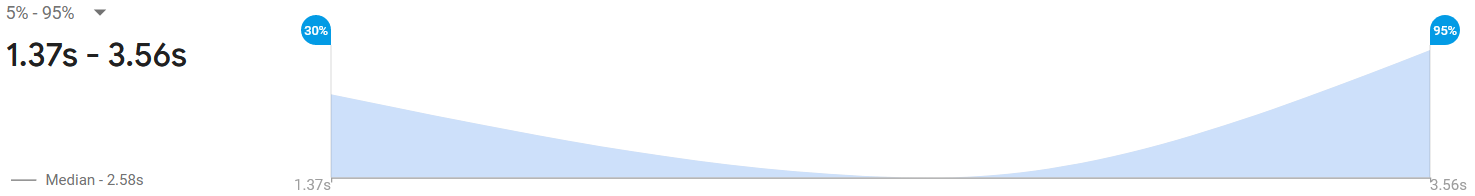
\includegraphics[height=0.1\textheight]{basisDuratieNative.png}
    \caption{Overzicht tijdsduur opstarten van applicatie met basisfunctionaliteiten bij Android.}
\end{figure}
Tijdens het meten van de duur voor het opstarten van de applicatie, 
is de applicatie meerdere keren opgestart. Op de grafiek is te zien dat de applicatie
gemiddeld 2,58 seconden nodig heeft om op te starten. Het minimum en maximum 
liggen op 1,37 en 3,56 seconden.

\paragraph{CPU \& geheugen}
\begin{figure}[H]
    \centering
    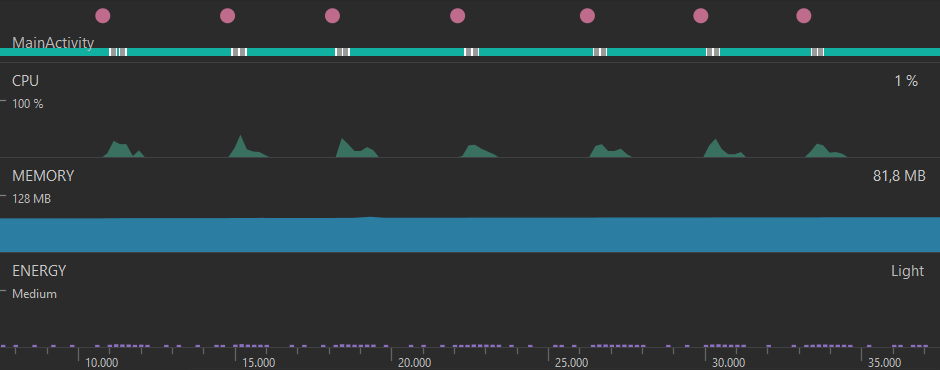
\includegraphics[height=0.25\textheight]{basisPerformantieNative.png}
    \caption{Overzicht CPU en geheugen gebruik tijdens het navigeren tussen schermen bij Android.}
\end{figure}
Op de grafiek is te zien dat het CPU gebruik van de applicatie wanneer deze 
inactief is, rond de 0 - 1\% ligt. En dat er duidelijk zichtbaar is wanneer er
genavigeerd wordt tussen de schermen. De piek van het CPU gebruik lag gemiddeld
op 31\% met een minimum en maximum van 25\% en 42\%. Het geheugen blijft in tegenstelling
met de CPU wanneer de applicatie inactief en actief is, rond de 81MB hangen, met
verschillen van maximum 2-3MB. Er is geen merkbaar verschil in het geheugen wanneer
er genavigeerd wordt tussen de schermen.

